\chapter{Fundamentação Teórica}
\label{chapter:fundamentos}

Nesta Seção são apresentados os conceitos base utilizados neste trabalho. Na Seção \ref{sec:lehmalaws}, são descriminadas as Leis de Lehman sobre Evolução de \textit{Software}. Na Seção \ref{sec:maintainability}, é apresentada uma breve descrição sobre conceitos de qualidade de \textit{software}. Na \ref{sec:softwareMetrics}, é apresentada a definição das métricas utilizadas no estudo.
\section{Evolução de software}
O termo \textit{evolução} descreve fenômenos observáveis em diferentes domínios, incluindo entidades ou conjuntos de entidades como espécies de seres vivos, sociedades, cidades, artefatos, conceitos, teorias e ideias. Se quaisquer destas mudanças são progressivas em alguma das suas qualidades, é dito que tais entidades \textit{evoluem} com o tempo. A mudança é definida como progressiva se puder ser considerada algum tipo melhoramento, podendo envolver ou não novas propriedades\cite{lehman1996laws}.

Muitas vezes, a mudança é motivada pela necessidade de adaptar a entidade individual ou a classe como um todo, para manter ou melhorar sua adequação dentro de circunstâncias ou contexto em mudança constante. A mudança nestas entidades pode tornar-las mais úteis ou significativas de alguma forma, ou incrementar seu valor de outras maneiras. Ela também pode remover propriedades não mais apropriadas. Mudanças fundamentais ou radicais, em geral, não são consideradas mudanças evolutivas, estas são geralmente incrementais e pequenas em relação a entidade ou classe em questão, mas exceções são possíveis.

Durante o seu ciclo de vida, sistemas de \textit{software} tipo E também passam por diversas mudanças, incrementos e mudanças de contexto, encaixando-se neste conceito de evolução. Este tipo de sistema foi observado e descrito pelas observações e dados adquiridos por Meir Lehman consistentemente por vários anos durante observações do sistema operacional OS/360-370, e posteriormente em outros sistemas \cite{lehman1979understanding,lehman1980programs,lehman1985program}. Os estudos revelaram similaridades no comportamento de crescimento de diferentes sistemas, sugerindo que sob as especifidades da evolução de cada sistema existe um fenômeno, ou seja, um processo de evolução comum que pode ser sistematicamente estudado e modelado. 

O processo de \textit{software} é concebido, direcionado, planejado, gerenciado e controlado por humanos. Em cada estágio do processo, supõe-se que as decisões direcionam as características do produto, tendo em vista que decisões de gerenciamento são diferentes de uma situação para a outra. Portanto, espera-se que comportamentos evolutivos variem significativamente entre aplicações, organizações, sistemas, tempo e lançamentos.

A descoberta de similaridades nos padrões de evolução num amplo conjunto de aplicações, desenvolvimento e marketing contradizem tais expectativas. Ao invés disto, as observações sugeriram que fatores similares entre os casos observados conduziram a evolução. 
 
Baseado em tais observações foram desenvolvidos modelos para descrever tais fenômenos, encapsulados em formas de Leis de Evolução de \textit{Software} \cite{lehman1985program}, descritas na seção seguinte.
\subsection{As Leis de Lehman sobre Evolução de Software} \label{sec:lehmalaws}

%Vários modelos presentes na literatura dividem o ciclo de vida do software em duas partes: o desenvolvimento até o lançamento inicial, e sua manutenção posterior. Porém, muitos sistemas reais, especialmente de tipo-E estão sujeitos à um desenvolvimento contínuo e continuam a evoluir durante sua existência. 
%Lehman estudou vários sistemas de larga escala e identificou as seguintes leis da evolução de software, descrevendo padrões comportamentais ao invés de questões técnicas\cite{lehman1979understanding,lehman1996laws}. Vários estudos proporcionaram suporte empírico as leis, em geral analisando como o tamanho do \textit{software} evolui com o tempo.

No fim dos anos 1960 e início dos anos 1970, Lehman e seus colaboradores foram os pioneiros em estudos empíricos em sistemas de \textit{software} após seu lançamento. Lehman e seu grupo examinaram uma série de sistemas proprietários(pertencentes a uma empresa ou organização, com código fechado), como o sistema operacional IBM 360-370. Ao fim dos anos 1970 e início dos anos 1980, o grupo também realizou observações em outros sistemas, focando no fenômeno da \textit{dinâmica de crescimento de grandes sistemas de \textit{software}}. Em suas observações, foi identificado não apenas que o \textit{software} muda, mas que também adquire novas funcionalidades, caracterizando segundo os autores, um processo de \textit{evolução de software}.

Lehman percebeu a evolução dos sistemas de \textit{software}, ou seja, sua mudança contínua, não era uma consequência de más praticas de programação, mas algo inevitavelmente necessário para manter o \textit{software} relevante perante a um domínio operacional em constante mudança e manter seus usuários satisfeitos. Tal ideia foi tão convincente que tal observação foi chamada de \textit{Lei} da mudança contínua, justificando o uso do termo \textit{lei} com base na afirmação que os desenvolvedores, individualmente, tem pouco controle do fenômeno. Outras observações empíricas foram encapsuladas em afirmações e também categorizadas com leis, sendo postuladas inicialmente apenas três seguidas de outras cinco leis adicionadas em trabalhos subsequentes, totalizando 8 leis.

Apesar da forte confiança na validade das leis, ainda não havia uma definição clara do seu escopo. Como contra exemplos, foram apresentados programas que depois de desenvolvidos são utilizados uma ou duas vezes e depois descartados. Assim, determinou-se que o primeiro requisito para a evolução de um \textit{software} é uma contínua necessidade do sistema, como por exemplo uma comunidade de usuários em que a utilização do programa possui algum valor. A análise de Lehman foi ainda além, argumentando que as leis aplicam-se apenas a categoria de sistemas de \textit{software} chamada por ele de sistemas \textit{tipo-E}\cite{lehman1979understanding}, em que o "tipo-E" caracteriza um sistema \textit{evolucionário}, em que o sistema tipo-E é aquele que aborda um problema (e portanto, seus requerimentos e sua especificação) que não pode ser completamente definido, tornando o \textit{software} sempre "incompleto" em algum aspecto por abordar problemas "em aberto", no sentido que seus requisitos podem sempre ser adicionalmente refinados ou modificados procurando satisfazer novas necessidades. Como consequência, há uma constante necessidade por mudanças e melhoramentos para um sistema de \textit{software} de tipo-E. Outra característica de sistemas de tipo-E é que sua utilização no seu domínio de operação muda o seu domínio, tornando-se assim um \textit{sistema de realimentação}, como ilustrado na Figura \ref{fig:feedbacksystem}. %TODO EXPLICAR IMAGEM

\begin{figure}
	\centering
	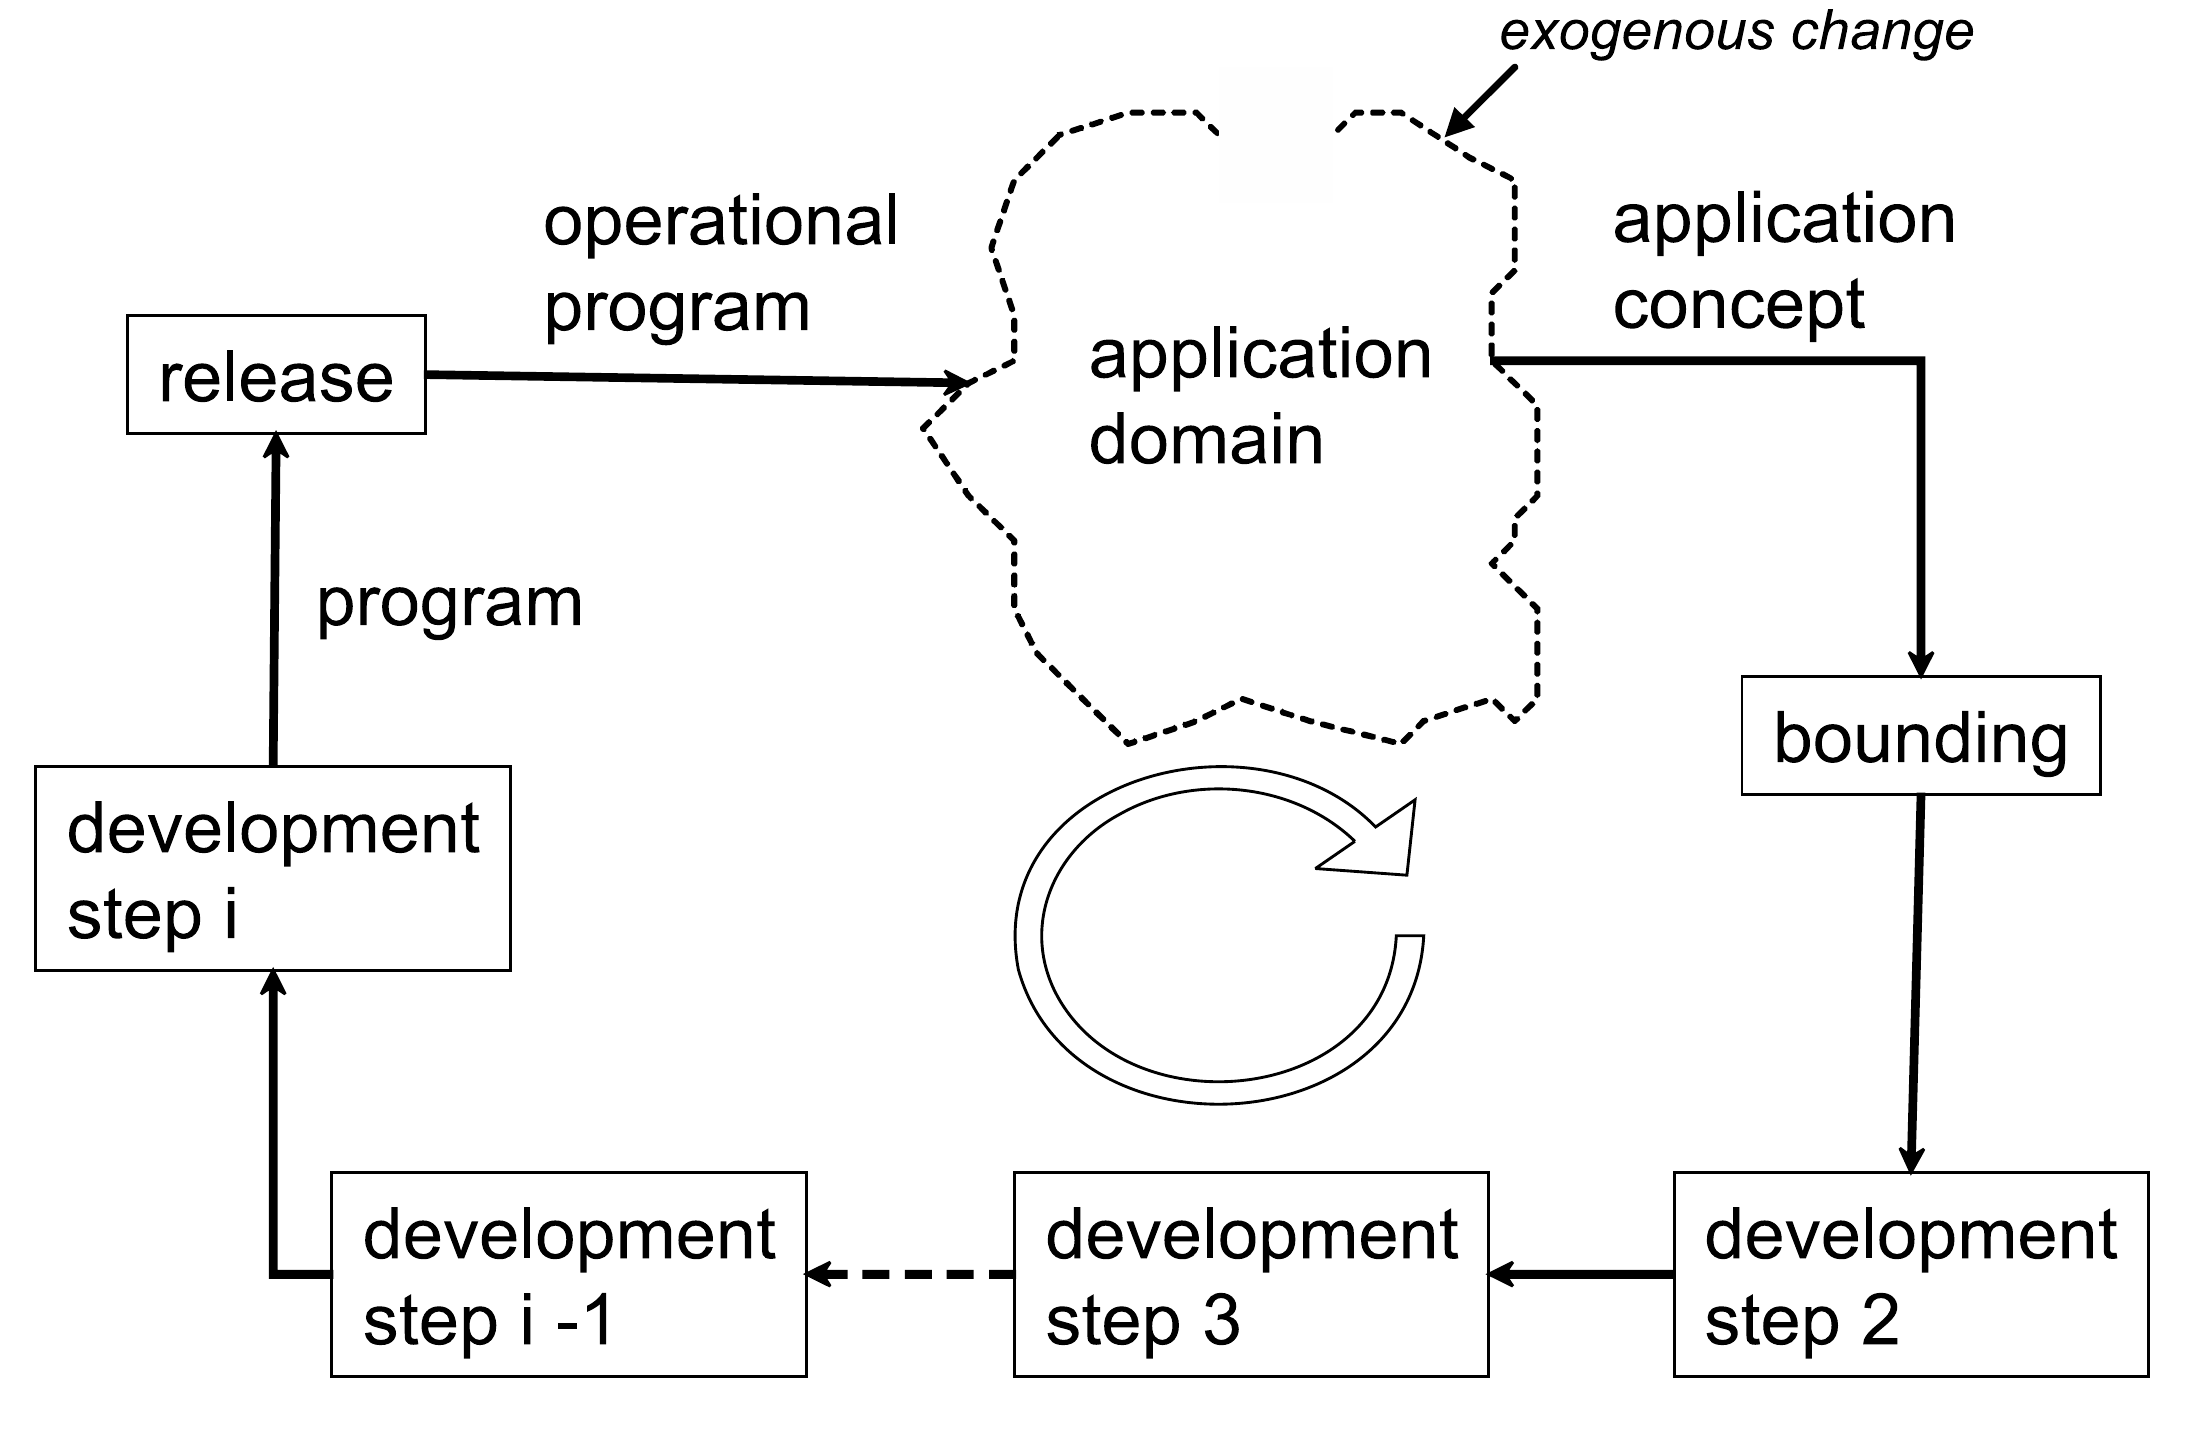
\includegraphics[width=0.7\linewidth]{figure/feedback_system}
	\caption{Processo de um Sistema de \textit{software} de tipo-E de acordo com a visão de Lehman, assim como apresentada em \cite{softwareEvolution2008}.}
	\label{fig:feedbacksystem}
\end{figure}

Lehman também classificou outros tipos de sistemas. Em contraste os sistemas de tipo-E, os sistemas de \textit{software} de \textit{tipo-S}, onde "S" representa \textit{especificado}(do inglês \textit{spefified}), possuem especificação completa e podem ser formalmente expressos através da matemática, utilizando provas para demonstrar que o programa satisfaz por inteiro sua especificação. Porém, a grande maioria dos sistemas utilizados em empresas e consumidores (como sistemas operacionais, processadores de texto, planilhas, navegadores de \textit{Internet}, sistemas de \textit{e-mail}) are encaixam-se no tipo-E\cite{softwareEvolution2008}, caracterizando assim a importância destes sistemas, assim como as leis que buscam caracterizar suas características evolutivas. 

Em sua classificação original\cite{lehman1979understanding}, Lehman também identificou um terceiro tipo de sistema, chamado de "P", representando \textit{problema}. Sistemas tipo-P são geralmente bem definidos e podem ser formalmente descritos, porém a sua abordagem baseia-se em heurísticas ao invés de provas matemáticas, como por exemplo sistemas de geração de horários para trens e voos. Se um sistema do tipo-P é ativamente utilizado, possivelmente irá adquirir algumas propriedades de sistemas do tipo-E, porém, tradicionalmente pesquisas em evolução de \textit{software} focam no naus comum, \textit{softwares} tipo-E.

Ao final dos anos 1990 e início dos anos 2000, novos estudos empíricos foram publicados por Lehman\cite{lehman2002overview} envolvendo cinco sistemas: o sistema de armas Matra-BAe, o núcleo do sistema operacional ICL VME, o sistema Logica FastWire e duas variantes do sistema de tempo real Lucent Technologies, levando ao refinamento das leis, tornando-as não mais afirmações isoladas e sim correlacionadas.

As leis de Lehman, na ordem em que foram formuladas são:
\begin{enumerate}
	\item \textit{Contínua Mudança }(1974): Um \textit{software} de tipo-E deve ser continuamente adaptado, ou tornará-se progressivamente menos satisfatório em uso. A adaptação refere-se as circunstâncias de uso do \textit{software}. Por exemplo, se uma prática de trabalho mudar, como uma mudança de procedimento ou uma nova metodologia de trabalho, sistemas de \textit{software} que auxiliam nestas práticas também devem mudar.
	\item \textit{Complexidade Crescente }(1974): A medida que o \textit{software} é alterado, sua complexidade estrutural tende a aumentar, sendo dificilmente reduzida ou mantida constante. Caso não haja esforço para manter e reduzir tal complexidade, a evolução do \textit{software} como um todo torna-se mais difícil(eg. reduz seu ritmo) ao longo do tempo. Esta lei complementa a primeira lei. Geralmente um programa é alterando visando a inserção, atualização ou remoção de uma das suas funcionalidades. Assim, as modificações podem ser realizadas diretamente em seu código, sem, no entanto, levar em consideração regras especificadas em sua arquitetura inicial. Isto implica que para manter o programa operacional, apenas investir na sua mudança não é suficiente. São necessários cuidados para manter o \textit{software} adequado a arquitetura inicial, permitindo que a complexidade permaneça em níveis aceitáveis e simplificando mudanças subsequentes.
	\item \textit{Auto-regulação }(1974): A evolução do \textit{software} é auto-regulada. Caracteriza-se em um equilíbrio entre demandas por mudanças (como novas funcionalidades, correções de problemas) e restrições pode ser feito dentro dos recursos disponíveis (como tempo). O passo da mudança passa assim a ser determinado, entre outros fatores, pela organização responsável pela manutenção. Assim, o \textit{software} auto-ajusta seu tamanho com incrementos e decrementos ao longo de sua evolução em concordância com os recursos disponíveis.
	\item \textit{Conservação da estabilidade organizacional(Quantidade de trabalho constante) }(1978): A quantidade de trabalho no desenvolvimento do \textit{software} tende a ser constante durante o tempo de vida operacional do \textit{software}. Segundo Lehman, isto reflete a dificuldade em mover membros da equipe entre locais de trabalho, fazer mudanças de orçamento, etc., caracterizando uma espécie de "inércia" em grandes organizações que produzem \textit{software}, ou seja, uma tendência a continuar trabalhando da mesma maneira. 
	\item \textit{Conservação de familiaridade }(1991): Em geral, o crescimento do \textit{software} tipo-E é restrito a necessidade mantê-lo familiar, pois desenvolvedores precisam entender o código fonte do programa e seu comportamento. Manter a familiaridade é importante tanto para desenvolvedores quanto para usuários. Grandes alterações num curto espaço de tempo aumentam a possibilidade de trazer problemas tais como defeitos, interações inesperadas, entre outros.
	\item \textit{Crescimento contínuo }(1991): As capacidades funcionais de sistemas de \textit{software} de tipo-E devem ser continuamente melhoradas para manter a satisfação do usuário durante a tempo de vida do \textit{software}. Esta é uma extensão da primeira lei: funcionalidade não é adaptada apenas para mudanças de condição, mas também incrementada com novas capacidades vindas de demandas de usuários e outros envolvidos com o \textit{software}.
	\item \textit{Qualidade decrescente }(1996): A menos que rigorosamente adaptado e evoluído para considerar mudanças operacionais do meio, a qualidade de um \textit{software} de tipo-E tende a diminuir. Esta lei é um corolário à primeira lei, e descreve os resultados de sua violação. Se o \textit{software} não é adaptado, premissas utilizadas durante a sua construção tornarão progressivamente menos relevantes ou até mesmo inválidas, e seus efeitos latentes podem ser imprevisíveis.
	\item \textit{Sistema de realimentação }(1996): Os processos da evolução do \textit{software} sistemas de avaliação com múltiplos níveis, loops e agentes. Múltiplos participantes estão envolvidos, incluindo gerentes, desenvolvedores, clientes e usuários. 
\end{enumerate}

Como uma sumarização, podemos dizer que quando aplicado a sistemas de \textit{software}, descreve o processo conduzido pelos desenvolvedores responsáveis pelo \textit{software} após seu lançamento inicial quando estes procuram introduzir correções (como consequências de más práticas de programação e outros defeitos), aperfeiçoamentos em funcionalidades e outras mudanças no \textit{software}, levando a um fenômeno de mudança gradual. 

Devido à definição informal das leis, ou seja, sem formalização de como podem ser verificadas, ficam abertas a interpretação em sua medição, assim como realizado em vários estudos \cite{lehman1985program,israeli2010linux,neamtiu2013towards}. Assim, é necessário a definição das propriedades mencionadas por Lehman, como qualidade e complexidade de \textit{software}, descritas na seções seguintes.
%Porém, grande parte dos estudos realizados durante quatro décadas na área utilizaram dados de sistemas proprietários. Com o surgimento de sistemas de \textit{software} \textit{open-source}, pode-se ter acesso a grandes massas de dados evolutivos disponíveis para estudo. Estudos iniciais sugeriram que sistemas \textit{open-source} evoluem em comportamentos diferentes dos esperados para sistemas proprietários.

%\subsection{A emergência de sistemas de \textit{software Open Source}
%
%Com o surgimento de 


%\subsection{Code Smells}

\section{Qualidade de software} \label {sec:softwareMetrics}
Nesta seção, é apresentada uma definição de qualidade de \textit{software} assim como definido no escopo deste trabalho.

A qualidade de \textit{software} produzido é uma das responsabilidades mais cruciais do desenvolvimento de um \textit{software}. A medida que a utilização de \textit{software }torna-se onipresente, garantir sua qualidade é uma preocupação crescente, porém, sua definição é um desafio desde o início da disciplina de engenharia de \textit{software}, levando a várias discussões e teorias ao redor do tema.

Qualidade de \textit{software} pode ser dividida em dois grupos principais: qualidades externas, visíveis aos usuários e pessoas que interagem com o sistema e qualidades internas, visíveis apenas para aqueles envolvidos no processo de desenvolvimento do \textit{software}.

Esta seção apresentará a qualidade interna utilizada para a análise dos projetos, a manutenibilidade de \textit{software}, definida nas seção a seguir.
\subsection{Manutenibilidade de Software} \label{sec:maintainability}
%TODO Transformar em Qualidade de Software
Manutenibilidade pode ser definida como a capacidade de modificação
do produto de \textit{software}. Modificações incluem correções, melhoramentos,
adaptações do \textit{software} para modificações no seu contexto, requerimentos
e especificações funcionais\cite{van1993software}.

Manutenção de \textit{software} é sempre necessária quando pretende-se que
um \textit{software} evolua com o tempo, adaptando-se ao contexto para o qual
foi construído ou perante ao não cumprimento de requerimentos, implicando
uma modificação no \textit{software} para que obtenha o comportamento correto.
Em \cite{brooks1995mythical}, o autor afirma: ``O custo total de manutenção de um \textit{software} largamente utilizado
é tipicamente 40\% ou mais do seu custo de desenvolvimento.''
Outros autores como em \cite{parikh1983tutorial}tem uma visão
mais pessimista, afirmando que de 45 à 60 porcento do tempo investido
em um \textit{software} é gasto em manutenção. Manutenibilidade é uma qualidade
cada vez mais valorizada por desenvolvedores no desenvolvimento e
gerenciamento de \textit{software}.

Projetos de \textit{software} livre dependem de contribuidores
para que continuem a evoluir, portanto, sua sobrevivência depende da
atração de novos contribuidores\cite{crowston2012free}. Possuir um
código com uma manutenibilidade comprometida torna o projeto mais
difícil de ser compreendido, dificultando a introdução de novos contribuidores.
Logo, manter uma boa manutenibilidade não é importante apenas para
o desenvolvimento, mas também para a atração de novos colaboradores.

Uma das abordagens mais comumente utilizadas para descrever o estado da manutenibilidade do código é a dívida técnica, descrita na seção seguinte.
\subsubsection{Dívida Técnica} \label{subsec:technical_debt}
A metáfora ``Dívida Técnica"(do inglês \textit{Technical Debt}) foi utilizada a primeira vez pelo programador americano Ward Cunningham para explicar à \textit{stakeholders} de perfil não-técnico a necessidade do que chamamos hoje de ``refatoração''. Segundo \cite{cunningham1993wycash}, a Dívida Técnica define-se como: 
\begin{quoteAbnt} Negligenciar o design é como pegar um empréstimo em dinheiro. Refatorar, é como pagar a dívida. O desenvolvimento retardado por conta da dívida pode ser visto como o pagamento dos juros no empréstimo. Cada minuto gasto em ``código-não-tão-correto'' conta com juros neste débito.\end{quoteAbnt}

Desde sua descrição original, o termo vêm sendo utilizado como uma forma de explicar os vários fatores de aumento de custos ao longo do ciclo de vida de um \textit{software} pela comunidade \cite{brown2010managing}.
Em certas situações, dívida não é necessariamente ``ruim'': uma pequena quantidade de dívida técnica pode ajudar desenvolvedores a acelerar o processo de desenvolvimento a curto prazo.
Em todo caso, as consequências podem ser notáveis a longo prazo se o projeto for de grande complexidade(o que pode implicar em dívidas onerosas), levando ao desenvolvimento mais lento e redução da produtividade.

Dívida técnica pode ser definida em várias dimensões diferentes, sintetizadas em \cite{tom2013exploration} como:
\begin{itemize}
	\item Dívida em código: A dívida técnica frequentemente manifesta-se na forma de código mal escrito - ``cada \textit{hack}, \textit{workaround} ou parte do código ruim acumula dívida técnica''\cite{stopford2010}. Como exemplos, podem ser citados duplicação e complexidade desnecessárias, estilo inadequado que reduz a facilidade de leitura do código ou lógica mal organizada que torna o \textit{software} suscetível falhas quando incrementado no futuro. Essencialmente, código que requer refatoração é uma forma de dívida em código.
	
	\item Dívida arquitetural e \textit{design}: Soluções rápidas de design e na arquitetura do projeto constituem outra forma de dívida técnica. Dívida de \textit{design} pode caracterizar-se na forma de uma solução rápida sem foco em atributos de qualidade, tais como manutenibilidade, adaptabilidade ou \textit{design} subsequente fragmentado sem que haja uma visão do todo\cite{shriver2010}. De forma análoga, débito arquitetural pode ser resultado de soluções rápidas sub-ótimas ou soluções que tornam-se insatisfatórias quando tecnologias ou padrões de projeto tornam-se obsoletos.
	
	\item Dívida de ambiente: Débito técnico pode também se manifestar no ambiente de uso da aplicação, que engloba processos relacionados ao desenvolvimento assim como \textit{hardware}, infraestrutura e aplicações de suporte. Processos manuais que podem ser automatizados são uma forma de dívida técnica que se acumula na forma de custo de trabalho manual, além da falta de exploração das potenciais melhorias oferecidas pela automação. Componentes ultrapassados do desenvolvimento da aplicação ou ambiente de operação também contribui para a dívida técnica. Como exemplos, temos vulnerabilidades de segurança ocasionadas pela postergação de atualizações na infraestrutura ou componentes que chegaram ao fim da sua vida útil.
	
	\item Dívida de distribuição de conhecimento e documentação: A falta da distribuição é outro aspecto da dívida técnica. Em \cite{slinker2008}, temos o seguinte exemplo:
	\begin{quoteAbnt}
		Um grande sistema com milhões de linhas de código pode ser mantido sem grandes gastos. Um dos fatores que mantém seu custo baixo é a permanência de seus desenvolvedores originais no sistema. Eles sabem porque e como tudo foi feito. Assim, a dívida é afetada pelos membros da equipe. Suponhamos que a mesma equipe fique insatisfeita por algum motivo e todos saiam da empresa. De repente, a dívida técnica mudou de baixa para extremamente elevada!
	\end{quoteAbnt}
	\item Dívida em testes:	Dívida técnica também pode representar a falta de testes levando a necessidade de testar manualmente o \textit{software} antes de cada lançamento ou cobertura de testes insuficiente independentemente se o os testes são automatizados ou não. A dívida em testes  pode incluir custos adicionais associados a danos à marca quando consumidores são afetados por falhas críticas, à necessidade de implementar correções em um ambiente de produção, diagnosticar e corrigir regressões, e a necessidade de execução de testes manuais quando automação não está disponível.
\end{itemize}

Em resumo, a dívida técnica pode ser caracterizada como a distância entre o estado atual do sistema de \textit{software} e um estado ``ideal'' hipotético no qual o sistema é adequado\cite{brown2010managing}, representando o custo ( seja em tempo de trabalho, pessoal, ou recursos financeiros) necessário para que tal estágio seja alcançado.
\subsection{Complexidade de Software}
Complexidade de \textit{software} é um produto natural do crescimento do número de recursos de um \textit{software}. Com múltiplas interfaces e requerimentos complexos, a complexidade do \textit{software} pode sair do controle tornando aplicações mais caras de serem mantidas e mais arriscado aprimora-las. Sem gerenciamento, a complexidade pode transformar aplicações em projetos difíceis de serem mantidos.

Complexidade excessiva pode impactar negativamente na habilidade do desenvolvedor de gerenciar interações entre camadas e componentes em uma aplicação. Também pode tornar módulos difíceis de serem incrementados e testados. Cada parte do código deve ser verificada para determinar como a mesma afetará a robustez e flexibilidade da aplicação. Complexidade de \textit{software} é uma das maiores preocupações de empresas que gerenciam diversas tecnologias e aplicações em uma arquitetura de vários níveis.

A engenharia de \textit{software} desenvolveu algumas medidas de complexidade \textit{software}, sendo a mais comum a medida de complexidade de McCabe, também chamada de complexidade ciclamática. 
\subsection{ Complexidade Ciclomática } \label{subsec:complexidade_ciclomatica}

Como complexidade pode ser um conceito subjetivo, \cite{mccabe1976complexity} definiu uma forma de mensurá-la. A complexidade ciclomática mede o número de caminhos de execução em uma aplicação. O cálculo é realizado através de conceitos da teoria dos grafos, descritos a seguir.

As seguintes definições da teoria dos grafos são necessárias:
\begin{definition}\thlabel{ciclomaticNumberDefinition}
O número ciclomático de um grafo F com n vértices e p componentes conexos é:
\end{definition}
\[ v(G) = e - n + p \]
\begin{theorem}
\thlabel{independentCircuitsTheorem}
Em um grafo fortemente conexo G, o número ciclomático é igual ao número máximo de circuitos independentes(ou seja, conjunto de vértices não adjacentes entre si). 
\end{theorem}

O teorema acima é aplicado da seguinte forma: dado um programa, um grafo direcionado é associado ao mesmo possuindo pontos de início e fim únicos(respectivamente o ponto de entrada do programa como uma diretiva \textit{begin}, e o ponto de saída como a diretiva \textit{end}). Cada nó no grafo corresponde a um bloco de código no programa onde há um fluxo sequencial e cada aresta corresponde a ramificações no programa. Tal grafo também é conhecido como grafo de fluxo de controle. Assume-se que cada nó pode ser alcançado partido do ponto de entrada, e todos os nós levam ao ponto de saída. Porém, grafos de controle de fluxo não são fortemente conexos. Para aplicarmos o \thref{independentCircuitsTheorem}, adicionamos um "arco virtual" a partir do nó de saída \textit{f} levando ao nó de entrada \textit{a}. O grafo de controle de fluxo G torna-se fortemente conexo(Em um grafo conexo, exite um caminho entre quaisquer dois vértices do grafo) tornando válida a aplicação do \thref{independentCircuitsTheorem}. A complexidade ciclomática é derivada do número ciclomático adicionando-se uma unidade representando-se a contribuição do arco virtual\cite{watson1996structured}. Tomando como exemplo o grafo G, com nove arestas e seis vértices, temos:
\[v(G) = 9 - 6 + 2 = 5\]
Na Figura \ref{fig:grafo-de-controle-de-fluxo}, há a representação de um grafo de fluxo de controle com o nó de entrada \textit{a} e o nó de saída \textit{f}. 
Assim, podemos escolher os seguintes circuitos independentes do em G:
\begin{verbatim}
B1: (abefa), (beb), (abea), (acfa), (adcfa).
\end{verbatim}
B1 forma a base para o conjunto de todos os circuitos em G e qualquer caminho em G pode ser expressado como uma combinação linear dos circuitos de B1. Por exemplo, o circuito \[(abeabebebef)\] pode ser expressado como \[(abea)+2(beb)+(abefa)\]. 

Ao usar o \thref{independentCircuitsTheorem} podemos escolher um conjunto base de circuitos que correspondem a caminhos no programa. O conjunto B2 é a base dos caminhos do programa.
\[B2: (abef).(abeabef),(abebef),(acf),(adcf)\]

A combinação linear dos caminhos em B2 também gera qualquer caminho. Por exemplo:

\[(abea(be)^3f) = 2(abebef) - (abef)\]


\begin{figure}
	\centering
	\includegraphics[width=0.35\linewidth]{../../controle_de_fluxo}
	\caption{Grafo G: Exemplo de grafo de controle de fluxo}
	\label{fig:grafo-de-controle-de-fluxo}
\end{figure}
\begin{figure}
	\centering
	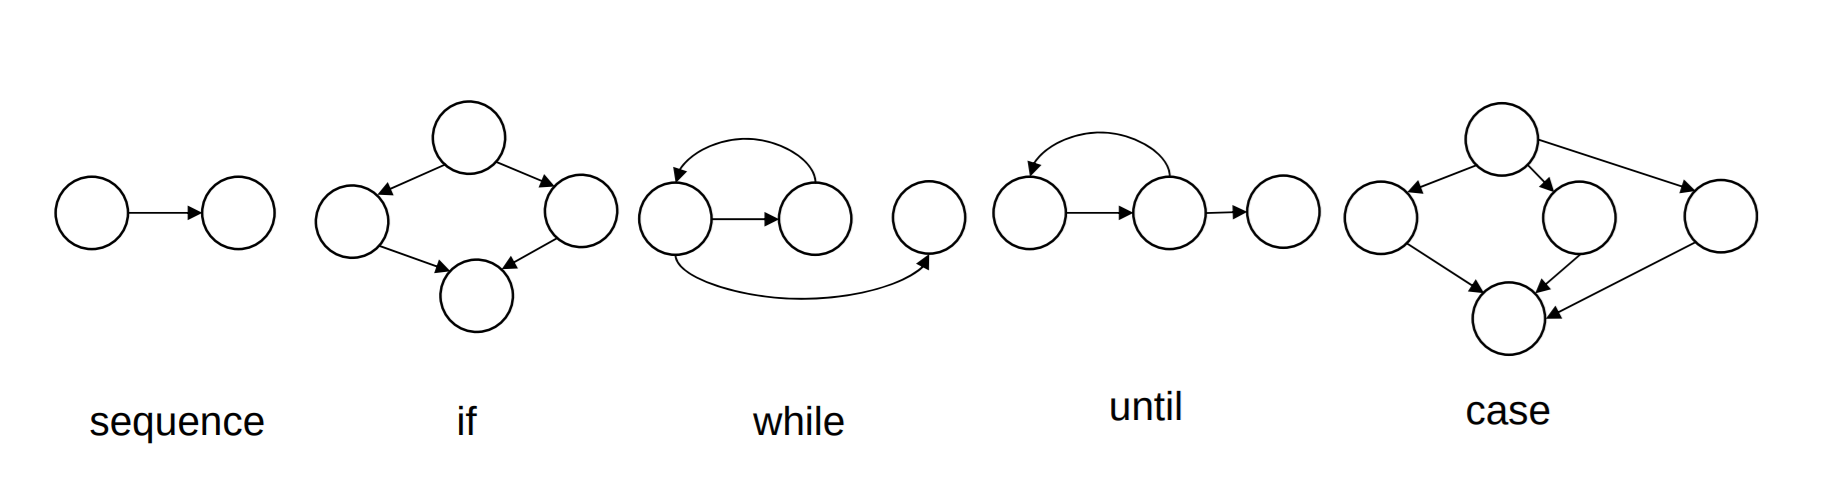
\includegraphics[width=0.5\linewidth]{figure/fluxo_estruturas}
	\caption{Representação de estruturas de controle em um grafo de controle de fluxo}
	\label{fig:fluxoestruturas}
\end{figure}

Para ilustrar melhor o relacionamento entre a complexidade ciclomática e o fluxo do programa, consideremos a Figura \ref{fig:fluxoestruturas}. Nela, uma sequência tem dois nós, um arco, um componente e portanto, contribui para uma complexidade de $C = 1 - 2 + 2$. Já a estrutura \textit{case} possui seis arcos, cinco nós e duas regiões, adicionando uma complexidade de $C = 6 - 5 + 2 = 3$.



%\subsection{O processo de desenvolvimento do Linux Kernel}
%
%Sendo um software livre, o desenvolvimento do Linux Kernel é público,
%mantido e gerenciado a partir do sistema de gerenciamento de configuração
%Git\cite{GitSCM2016}. Qualquer desenvolvedor pode contribuir para
%o projeto. Neste contexto, chama-se de desenvolvedor qualquer pessoa
%que envia um \emph{patch}(conjunto de modificações em um arquivo,
%geradas pelo software de controle de versão \emph{Git}) para o projeto.
%A organização do projeto é realizada através da \emph{Linux Kernel
%Mailing List}(LKML)\cite{lkml2016}\emph{, }uma lista de discussão
%onde os desenvolvedores podem comunicar-se e enviar suas contribuições.
%Todas as contribuições devem ser enviadas através da LKML.
%
%Uma visão geral da estrutura do desenvolvimento é mostrada na Figura
%\ref{fig:Estrutura-Organizacional}.Para distribuir a organização
%do projeto, alguns desenvolvedores são responsáveis pela manutenção
%de partes do sistema, sendo chamados de mantenedores. Todo arquivo
%do projeto possui um mantenedor e faz parte de um conjunto maior,
%chamado subsistema. Subsistemas agrupam partes do projeto com funcionalidades
%relacionadas como comunicação de rede, \emph{drivers, }sistemas de
%arquivos, entre outros. Todo subsistema é também possui um mantenedor
%responsável.
%
%\begin{figure}[H]
%\begin{centering}
%\includegraphics[clip,width=0.7\paperwidth]{\string"figure/Linux Development Structure\string".png}
%\par\end{centering}
%\caption{Estrutura organizacional do Linux Kernel}
%\label{fig:Estrutura-Organizacional}
%\end{figure}
%
%Qualquer desenvolvedor pode enviar contribuições para qualquer arquivo
%do projeto. Sua contribuição pode ser enviada através da LKML, enviando
%o \emph{patch} ao mantenedor do arquivo o qual as contribuições dizem
%respeito. Posteriormente, o mantenedor revisa o que foi enviado e
%decide se a contribuição pode ser incorporada ao projeto. Como critério
%de avaliação, o mantenedor leva em conta orientações de estilo de
%código próprias do projeto\cite{codingstyle2016}. Caso a contribuição
%seja aceita, ela é enviada ao mantenedor do subsistema o qual o arquivo
%pertence. Quando o mantenedor do arquivo envia a contribuição para
%o mantenedor do subsistema, ele adiciona sua ``assinatura'' informando
%que tal \emph{patch }foi revisado por ele.
%
%Durante o processo, os repositórios dos subsistemas( repositórios
%Git) são unificados, em um repositório chamado de \emph{linux-next}.
%Assim, contribuições de diferentes subsistemas podem ser unidas e
%testadas em conjunto. No topo do processo, encontra-se Linus Torvalds,
%criador do projeto, para onde os mantenedores dos subsistemas enviam
%as alterações que possuem.
%
%Todo o processo é construído baseado na chamada ``cadeia de confiança''.
%Torvalds cofia nos mantenedores dos subsistemas, que por sua vez confiam
%nos mantenedores dos arquivos. Isso não significa que é esperado que
%os mantenedores não cometam erros, mas sim estarão disponíveis para
%resolver quaisquer problemas provenientes de oriundos de contribuições
%que aprovaram durante o ciclo.
%
%Com esta estrutura hierárquica garante, segundo os membros do projeto,
%que toda contribuição é revisada por pelo menos duas pessoas: a que
%a escreveu e a que a assinou. Assim, os desenvolvedores manter o projeto
%dentro dos padrões estabelecidos, evitando a degradação da manutenibilidade
%do código.
%
%\subsection{O método SQALE}
%
%O método SQALE (Software Quality Assessment based on Life Cycle Expectations)
%tem como objetivo oferecer uma análise da qualidade do código fonte
%da forma mais objetiva possível, e com o menor número possível de
%``falsos positivos''. Para SQALE, avaliar a qualidade de uma aplicação
%significa medir seu Débito Técnico. Débito Técnico é uma metáfora
%usada pela primeira vez por Ward Cunningham\cite{cunningham1993wycash}.
%Sua definição pode ser sumarizada citando-o:
%\begin{quote}
%\emph{``Negligenciar o design é como pegar um empréstimo em dinheiro.
%Refatorar, é como pagar o débito. O desenvolvimento retardado por
%conta do débito pode ser visto como o pagamento dos juros no empréstimo.
%Cada minuto gasto em ``código-não-tão-correto'' conta com juros
%neste débito.''}
%\end{quote}
%Para SQALE, a definição do Débito Técnico significa o custo necessário
%para adequar o código fonte de um software de um determinado estado
%à sua qualidade objetivo. Tal objetivo é definido pelo modelo de qualidade
%através das características, sub-características e requerimentos,
%definidos a seguir.
%
%O método define 4 conceitos chave, descritos brevemente a seguir e
%detalhados nas seções subsequentes:
%\begin{enumerate}
%\item \textbf{O modelo de qualidade: }O Modelo de Qualidade SQALE é utilizado
%para formular e organizar os requerimentos não-funcionais relacionados
%a qualidade do código. O modelo é organizado em três níveis hierárquicos.
%O primeiro nível é composto de características, o segundo de sub-características,
%e o terceiro nível é composto de requerimentos relacionados aos atributos
%internos do código fonte. Tais requerimentos variam de acordo com
%o contexto e linguagem de programação utilizada\cite{letouzey2012sqale}.
%\item \textbf{O Modelo de Análise: }O Modelo de Análise SQALE contém regras
%utilizadas para normalizar as medições e violações relacionadas ao
%código, além de outras regras para agregar os valores normalizados.
%\item \textbf{Os Índices: }Todos os índices representam custos. Um índice
%é representa o débito técnico total do projeto. Os outros índices
%utilizados, são utilizados para analisar tal débito.
%\item \textbf{Os Indicadores: }O método define três indicadores sumarizados.
%Estes são utilizados como representação visual do Débito Técnico.
%\end{enumerate}
%Adicionalmente a tais conceitos, o método define 8 princípios sumarizados
%em 3 itens, que visam obter uma estimativa precisa do Débito Técnico:
%\begin{itemize}
%\item Qualidade significa adequação aos requerimentos. Portanto, tais requerimentos
%devem ser previamente definidos.
%\item O método analisa a distância de adequação aos requerimentos, considerando
%o custo de remediação necessário para trazer o código à conformidade.
%\item O método soma todos os custos de remediação para calcular os indicadores
%de qualidade.
%\end{itemize}
%O método é detalhado nos parágrafos seguintes.
%
%\subsubsection{O Modelo de Qualidade SQALE}
%
%O modelo de qualidade do método SQALE contém propriedades internas
%desejadas do código, no contexto da avaliação. Em outras palavras,
%SQALE requer que projetos ou organizações estabeleçam sua própria
%definição concreta de ``código correto''. Desta forma, pode-se definir
%de forma clara em seus respectivos contextos o que é gera débito ou
%não.
%
%A definição de código correto tipicamente inclui nível de implementação,
%e convenções de nomenclatura e apresentação. Também devem ser inclusos
%requerimentos arquiteturais e estruturais. Este modelo possui 4 propriedades
%importantes:
%\begin{itemize}
%\item Este é um modelo de requerimentos, não um conjunto de melhores práticas
%de implementação.
%\item O modelo é construído levando em conta o ciclo de vida do código fonte.
%\item É estruturado em níveis hierárquicos.
%\item Leva em conta tanto o ponto de vista do desenvolvedor quando do usuário.
%\end{itemize}
%As características básicas do modelo são definidas com base no ciclo
%de desenvolvimento de um arquivo contendo código fonte. Tal organização
%dos requerimentos é organizada sequencialmente como representada da
%Figura \ref{N=0000EDveis-Sqale} dos níveis mais baixos como a ação
%de escrita do código, testes, modificações e as qualidades associadas
%a cada ação.
%
%O modelo em camadas apresentado na Figura \ref{N=0000EDveis do modelo SQALE}
%é o resultado final desta abordagem. O modelo pode ser adaptado levando
%em conta o ciclo de vida do código fonte a ser analisado.
%
%\begin{figure}
%\begin{centering}
%\includegraphics[width=0.7\paperwidth]{\string"figure/O ciclo de vida SQALE\string".png}
%\par\end{centering}
%\centering{}\caption{Ciclo de desenvolvimento de arquivo no modelo de qualidade SQALE}
%\label{N=0000EDveis-Sqale}
%\end{figure}
%
%Nesta estrutura, uma sub-característica ou um requerimento nunca é
%duplicado em nenhum nível. Utilizando um requerimento e uma sub-característica
%apenas uma vez é uma regra essencial do Modelo de Qualidade SQALE.
%Esta regra se aplica para qualquer requerimento identificado na definição
%de ``código correto''. A Figura \ref{N=0000EDveis 2 e 3}, é mostrado
%um exemplo com requerimentos dizendo respeito a determinadas sub-características,
%também relacionadas a uma característica.
%
%
%\subsubsection{O Modelo Análise SQALE}
%
%Como descrito anteriormente, para o método SQALE analisar o código
%fonte é análogo a medir a distância do estado no código durante a
%medição à sua qualidade objetivo. Esta distância permite normalizar
%toas as medições internas em uma escala comum. Para realizar a medição,
%o Modelo de Analise SQALE utiliza um índice de remediação associado
%a cada componente do código fonte (módulos, arquivos ou classes).
%O índice de remediação representa o custo das ações de remediação
%necessárias para corrigir as violações detectadas no componente, em
%relação aos requerimentos do modelo. Como o tal índice representa
%um custo, a consolidação dos índices consiste na adição de informações
%uniformes.
%
%\begin{table}
%\begin{centering}
%\begin{tabular}{|>{\centering}p{0.15\textheight}|c|>{\centering}p{0.1\textheight}|}
%\hline 
%Requerimento & Detalhes da Remediação & Função de Remediação\tabularnewline
%\hline 
%\hline 
%Não há bloco de instrução comentado. & Remover, não há impacto no código compilado & 2 minutos por ocorrência\tabularnewline
%\hline 
%A indentação do código deve seguir uma padrão consistente & Ajustar com auxílio de recursos de IDEs & 2 minutos por ocorrência\tabularnewline
%\hline 
%Código deve sobrescrever tanto o método ``equals'' quanto ``hashcode'' & Escrever código e teste & 1h por ocorrência\tabularnewline
%\hline 
%Todos os arquivos possuem pelo menos 70\% de cobertura de testes & Escrever testes adicionais & 20 minutos por linha não não coberta para alcançar 70\% de cobertura\tabularnewline
%\hline 
%Não há trechos clonados de 100 palavras ou mais & Refatorar com IDE e escrever testes & 20 minutos por ocorrência\tabularnewline
%\hline 
%\end{tabular}
%\par\end{centering}
%\caption{Exemplo de Funções de Remediação}
%\label{Tabela de remedia=0000E7=0000E3o}
%\end{table}
%
%Custos de remediação são calculados associando-se Funções de Remediação
%a todos os requerimentos do Modelo de Qualidade. Estas devem ser estabelecidas
%e calibradas pelo projeto ou organização. Elas dependem principalmente
%nas atividades necessárias para resolver uma violação. Por exemplo,
%ajustar uma linha de código com indentação incorreta leva o mesmo
%esforço de corrigir um defeito estrutural do código. O conjunto completo
%das Funções de remediação é um Modelo de estimativa de Débito Técnico.
%A Tabela \ref{Tabela de remedia=0000E7=0000E3o} mostra um exemplo
%de funções de remediação, com as unidades representadas em tempo de
%desenvolvimento. Cada requerimento, como o ``Não há um bloco de instrução
%comentado'' possui uma remediação detalhada e um tempo estimado de
%remediação, dado pela Função de Remediação.
%
%\begin{figure}
%\begin{centering}
%\includegraphics[width=0.7\paperwidth]{\string"figure/Exemplo de remediacao\string".png}
%\par\end{centering}
%\centering{}\caption{Ciclo de desenvolvimento de arquivo no modelo de qualidade SQALE}
%\label{Exemplo de calculo de remedia=0000E7=0000E3o}
%\end{figure}
%
%
%\subsubsection{Os Índices SQALE}
%
%O índice mais importante definido pelo método é o índice de qualidade
%global: para cada elemento dos artefatos do código fonte, o índice
%de remediação relacionado a todas as características do Modelo de
%Qualidade podem ser estimadas adicionando todos os índices de remediação
%relacionados a todos os requerimentos do Modelo de Qualidade. Tal
%índice é chamado de Indice de Qualidade SQALE(SQI). O SQI representa
%o Débito Técnico do código fonte analisado. A precisão do resultado
%dependo do nível de detalhes das Funções de Remediação definidas.
%
%Os índices de remediação e o Débito Técnico podem ser calculados em
%unidades de tempo, esforço ou unidades monetárias.
%
%Para cada elemento dos artefatos do código fonte, o custo de remediação
%relacionado a uma determinada característica pode ser estimado somando
%todos os índices de remediação para os requerimentos da característica.
%Os índices das características SQALE são os seguintes:
%\begin{itemize}
%\item Índice de Testabilidade: STI
%\item Índice de Confiabilidade: SRI
%\item Índice de Mutabilidade: SCI
%\item Índice de Eficiência: SEI
%\item Índice de Segurança: SSI
%\item Índice de Manutenibilidade: SMI
%\item Índice de Portabilidade: SPI
%\item Índice de Reusabilidade: SRuI
%\end{itemize}
%\begin{figure}
%\begin{centering}
%\includegraphics[width=0.7\paperwidth]{\string"Niveis 2 e 3 do modelo SQALE\string".png}
%\par\end{centering}
%\centering{}\caption{Detalhes dos níveis 2 e 3 do Modelo de Qualidade SQALE}
%\label{N=0000EDveis 2 e 3}
%\end{figure}
%
%O método também define índices de densidade como a densidade de Débito
%Técnico, que permite a comparação do Débito Técnico de produtos de
%diferentes tamanhos.
%
%\subsubsection{Indicadores SQALE}
%
%O método também define indicadores, úteis para análise. Neste trabalhos
%focamos apenas no indicador de Classificação. O indicador de Classificação
%oferece uma abstração de mais alto nível baseada na razão entre o
%Débito Técnico e o custo de desenvolvimento. O método requer a definição
%de uma escala, como a apresentada na Figura \ref{Escala SQALE}. A
%escala divide a classificação em 5 níveis, sendo melhor classificados
%aqueles com a menor razão entre o Débito Técnico e o custo de desenvolvimento.
%
%\begin{figure}
%\begin{centering}
%\includegraphics{\string"Escala SQALE\string".png}
%\par\end{centering}
%\centering{}\caption{Exemplo de Escala SQALE}
%\label{Escala SQALE}
%\end{figure}
%
%
%\subsection{Ferramentas de Análise utilizadas.}
%
%Para realizar a análise, foram utilizados o software SonarQube\cite{SonarQube2016}.
%O SonarQube é uma plataforma de qualidade de código open source, que
%oferece uma imagem da qualidade do código. A ferramenta é utilizada
%por mais de 50.000 empresas em todo mundo, com cerca de 2 milhões
%de usuários\cite{SonarQubeUsage2016}. O SonarQube possui diversas
%análises, mas focamos nossa análise na sua avaliação da manutenibilidade,
%que utiliza o método SQALE para avaliação de débito técnico. A Tabela
%\ref{M=0000E9tricasSonarQube} descreve as métricas utilizadas pelo
%software, como sua definição de indicadores e método de cálculo de
%razão de débito técnico.
%
%\begin{table}
%\begin{centering}
%\begin{tabular}{|c|>{\centering}p{0.6\textwidth}|}
%\hline 
%Nome & Descrição\tabularnewline
%\hline 
%\hline 
%\emph{Code smells} & Número de ``\emph{Code Smells}'' encontrado\tabularnewline
%\hline 
%Classificação dos Indicadores. & Classificação dada a um projeto relacionada a razão do débito técnico.
%
%A escala é definida como:
%
%A=0-0.05, B=0.06-0.1, C=0.11-0.20, D=0.21-0.5, E=0.51-1
%
%Em outras palavras, pode-se dizer que o custo de remediação total 
%
%é:
%\begin{itemize}
%\item <= 5\% Do tempo que já foi investido na aplicação, sua classificação
%é A
%\item Entre 6\% e 10\%, B
%\item Entre 11\% e 20\%, C
%\item Entre 21\% e 50\%, D
%\item Qualquer valor acima de 50\%, E
%\end{itemize}
%\tabularnewline
%\hline 
%Débito Técnico & Esforço necessário para resolver todos os problemas de manutenibilidade,
%armazenados em minutos.\tabularnewline
%\hline 
%Razão do débito Técnico & \begin{raggedright}
%Razão entre o custo de desenvolvimento do software e o custo para
%resolver seus problemas. A formula para calculo é:
%\par\end{raggedright}
%\begin{quote}
%Custo de Remediação / Custo de Desenvolvimento
%\end{quote}
%\begin{raggedright}
%Podendo ser reescrito como:
%\par\end{raggedright}
%\begin{quote}
%Custo de Remediação /(Custo de desenvolvimento de 1 linha de código
%{*} Numero de linhas de código)
%\end{quote}
%\raggedright{}O valor do custo para desenvolver uma linha de código
%é definido como 0.06 dias.\tabularnewline
%\hline 
%\end{tabular}
%\par\end{centering}
%\caption{Métricas do SonarQube}
%\label{M=0000E9tricasSonarQube}
%\end{table}
%
%O SonarQube utiliza também os chamados \emph{Code Smells} para o avaliação
%da manutenibilidade. \emph{Code Smells} são sintomas no código fonte
%de um programa que possivelmente indicam problemas mais profundos,
%como indução a erros de programação ou possibilidades de comportamento
%inesperado. Estes são fatores importantes que contribuem com o Débito
%Técnico e possivelmente afetando negativamente a manutenibilidade
%do código\cite{tufano2015and}.